\begin{multicols}{3}[\section{5G}]

\rhead{Autor: Lucas Lorenz}
\lfoot{Letzte Bearbeitung: 17.04.2016}

\newrefsegment

\begin{boxedminipage}{\linewidth}
\begin{tabular}{p{2,1 cm}p{2.7 cm}}
\textbf{Steckbrief}& \\
\end{tabular}
\begin{tabular}{p{2,1 cm}|p{2.7 cm}}
      Einsatz ab & voraussichtlich 2020\\
      \hline
      Frequenz"-bereich  & mm-Band (\SI{24.25}{\giga\hertz}-\SI{86}{\giga\hertz}) oder C-Band (\SI{3.4}{\giga\hertz}-\SI{3.8}{\giga\hertz}) \cite{5g.8}\\
      \hline
      Datenrate & \SI{10}{\giga bit/\second}\\
      \hline
      Verbreitung & In Entwicklung\\
      \hline
      Reichweite & etwa \SI{100}{\metre} bis \SI{2}{\kilo\metre} \\
\end{tabular}
\end{boxedminipage}
\par
%Source http://www.fh-bingen.de/fileadmin/user_upload/Lehrende/Kilsch_Dieter/internet/projekte/TedoSchStiUnits.pdf -> Seite 9 findet ihr alle verwendbaren Einheiten, wie:
%\SI{Zahl}{\mega\hertz} oder \SI{Zahl}{\mili\metre}
%Ich weiß ehrlich gesagt nicht welche Einheiten ihr im Text genau braucht, aber in dem Dokument und mit obigen Beispiel sollte es umsetzbar ein.
\subsection*{Überblick}
5G (eng. Abkürzung für fifth-generation) ist der Name für die fünfte Generation der Telekommunikationstechnologie, die sich noch in einem frühen Stadium der Entwicklung befindet. Dabei geht es darum die am besten geeigneten Frequenzbereiche für die Datenübertragung zu finden und die Technik zu testen sowie entsprechende Geräte und Adapter zu konstruieren.

Grundlegende Ziele im Vergleich zu 4G sind:\cite{5g.6}
\begin{itemize}
\item \si{100}fach erhöhte Übertragungsgeschwindigkeit
\item \si{1000}fach größere Datenkapazität
\item verringerte Latenzzeiten von unter \SI{1}{\milli\second}
\item erheblich geringerer Energieverbrauch 
\item bessere Ausnutzung des vorhandenen Frequenzspektrums
\end{itemize}
Damit sollen unter anderem auch eine erweiterte Machine-2-Machine-Kommunikation (M2M-Kommunikation) unterstützt werden, darunter besonders die flächendeckende Ermöglichung von selbstfahrenden Autos, welche in ihrer Echtzeitumgebung besonders stark auf geringe Latenzzeiten angewiesen sind. \cite{5g.1}
\subsection*{Technische Erläuterungen}
Da die Technologie hinter 5G noch in der Entwicklungsphase ist und noch keine Standardisierung festgelegt wurde, und da verschiedene Ansichten exisitieren, was genau 5G wirklich bedeutet, existieren auch noch keine präzisen Kenntnisse über die zugrundeliegende Technik.
Um allerdings die bereits angesprochenen Ziele von 5G zu erreichen, müssen verschiedene Grundlagen auf Seiten der Technik gewährleistet werden, welche stattdessen an dieser Stelle erläutert werden.

\begin{Figure}
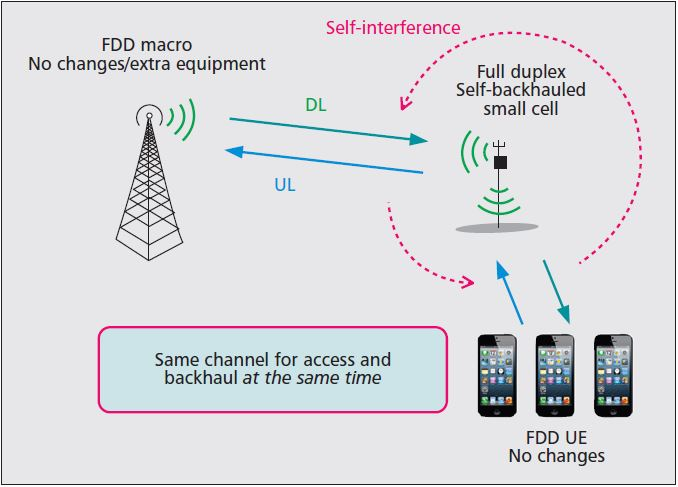
\includegraphics[width=\linewidth]{Kapitel/5G/Grafiken/sic}
\captionof{figure}{Nutzung von gleichen Frequenzen für Uplink und Downlink durch Mobilfunknetzzelle ~\cite{5g.7}}
\label{fig:5g.sic}
\end{Figure}

Die beste Ausnutzung des Frequenzspektrums kann nur mithilfe von Vollduplex (IBFD = In Band Full Duplex) erreicht werden, das heißt, dass zeitgleich auf der gleichen Frequenz gesendet und empfangen wird.
Unter Ausnutzung von IBFD kann also das Frequenzspektrum doppelt so effektiv genutzt werden wie bisher. Damit einher geht direkt, dass sich die Menge der übertragbaren Daten auf den Frequenzbereich hin betrachtet, sprich die Kapazität des Netzes, ebenfalls verdoppelt.
IBFD wurde im September 2015 zum ersten Mal von der Telekom durch die Nutzung von Selbstinterferenzunterdrückung (SIC = Self Interference Cancellation) erreicht.

Im Fall in Abbildung \ref{fig:5g.sic} wird SIC dadurch erreicht, dass die Netzzelle auf einer Frequenz vom Funkmast Daten erhält und auf dieser auch Daten an die einzelnen Endgeräte sendet. Zeitgleich empfängt sie auf einer zweiten Frequenz von den Endgeräten und sendet auf dieser auch an den Funkmast, sodass die Interferenz aufgehoben wird.

\begin{Figure}
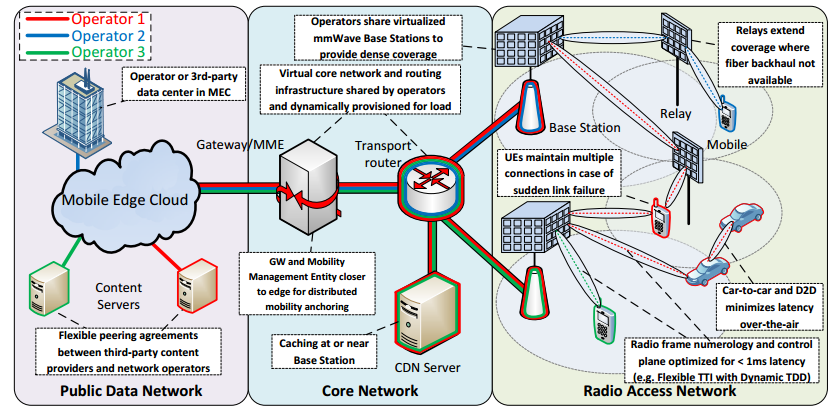
\includegraphics[width=\linewidth]{Kapitel/5G/Grafiken/5g-changes}
\captionof{figure}{Notwendige Veränderung am Netzwerk für möglichst geringe Latenzzeiten ~\cite{5g.9}}
\label{fig:5g.changes}
\end{Figure}

Um Latenzzeiten von weniger als \SI{1}{\milli\second} zu erreichen, 
%welche unter anderem für den Einsatz von selbstfahrenden Autos als notwendig angesehen werden, um die Sicherheit zu gewährleisten, 
müssen Veränderungen am ganzen Netzwerk vorgenommen werden, wie sie in Abbildung \ref{fig:5g.changes} aufgezeigt sind.
Darüber hinaus wird stark in Betracht gezogen, einen höheren Frequenzbereich für die Datenübertragung zu nutzen als jemals zuvor, etwa im Bereich der Millimeter-Wellen, also mit zwischen \SI{20}{\giga\hertz} und \SI{80}{\giga\hertz}. Dadurch kann schneller mit der Datenübertragung und dem Empfang begonnen werden, sodass auch hier an kritischer Zeit gespart wird.
\subsection*{Einsatzmöglichkeiten}
Die Einsatzmöglichkeiten von 5G hängen besonders von 3 Eigenschaftes des Netzwerks ab:
\begin{itemize}
\item Anzahl der maximalen Verbindungen
\item Latenzzeit
\item Übertragungsgeschwindigkeit
\end{itemize}

Dabei stellen einige Anwendungen ganz spezielle Anforderungen an das Netzwerk und die Technik, während andere weniger harte Kriterien aufweisen.

Wie auch aus Abbildung \ref{fig:5g.aw} hervorgeht, ist die Anzahl der Verbindungen die hauptsächlich definierende Größe, wenn es um Thematiken wie das Internet der Dinge und den zunehmenden Einsatz von Sensoren, auch im privaten Umfeld, geht.
Hier muss jedes Gerät stets mit dem Netzwerk in Verbindung stehen, um möglichst selbstständig präzise Entscheidungen treffen zu können. Beispielsweise kann der Kühlschrank einer Person dieser direkt mitteilen, dass die Milch fast alle ist, und die Person kann so direkt nach der Arbeit einkaufen gehen.

\begin{Figure}
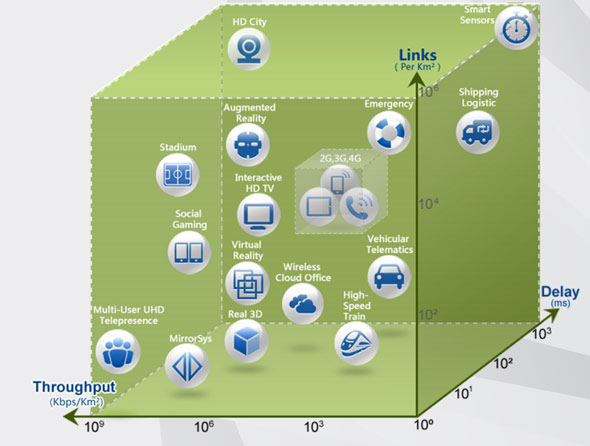
\includegraphics[width=\linewidth]{Kapitel/5G/Grafiken/5g-anwendung}
\captionof{figure}{5G-Anwendungswürfel von Huawei ~\cite{5g.6}}
\label{fig:5g.aw}
\end{Figure}

Auch beim Einsatz von Sensoren im privaten Umfeld, das heißt speziell die Überwachung der Körperfunktionen und Umgebung eines Nutzers, muss jeder Sensor in Echtzeit in Kontakt stehen mit beispielsweise dem Smartphone oder einem zentralen System, welches die Daten dann sammeln und auswerten könnte. Damit könnten frühzeitig drohende Gefahren für die Gesundheit wie Herzinfarkte erkannt werden. Darüber hinaus könnte mit den Sensordaten auch Hinweise zu einer gesünderen Lebensweise gegeben werden, um etwa Mineralmangel vorzubeugen, oder der Schlafrythmus könnte entsprechend der Schlafphasen optimiert werden.

Um 5G auch als großflächiges Mobilnetzwerk nutzen zu können, werden bald neue Übertragungsgeschwindigkeiten notwendig sein. Wenn Videos in 4K und 3D nichtmehr die Ausnahme sind oder Nutzer die Vorteile von Virtual Reality (VR) im Alltag ausnutzen wollen, dann werden die aktuellen Geschwindigkeiten schnell an ihre Grenzen stoßen.
Beispielsweise benötigt das Bild, um echte VR zu erreichen, mindestens so viele Daten, wie die menschliche Retina erfassen kann. Um dies zur Verfügung zu stellen, werden über \SI{300}{\mega bit/\second} benötigt, was 4G-Netze schlicht nicht leisten können.
Durch Nutzung dieser Technik wäre es allerdings möglich, beispielsweise die Lernmöglichkeiten in virtuellen Klassenräumen extrem auszubauen, was auch für Kinder in Gegenden wie im australischen Outback sehr hilfreich sein könnte.

Wenn vom Netz eine Latenzzeit von weniger als \SI{1}{\milli\second} gewährleistet werden kann, werden dadurch neue Möglichkeiten in der Automobiltechnik und der Medizin gegeben sein.

In der Automobiltechnik sind die Latenzzeiten von so hoher Bedeutung, da sich ein selbstfahrendes Auto unter Nutzung des aktuellen 4G-Netzes mit Latenzen von \SI{50}{\milli\second} bei \SI{100}{\kilo\metre /\hour} noch \SI{1.4}{\metre} bewegen würde, bevor es zu bremsen beginnt. Mit der angestrebten Latenzzeit von 5G könnte diese Strecke auf \SI{2.8}{\centi\metre} reduziert werden, was mit der Reaktionsgeschwindigkeit des ABS vergleichbar ist.

Außerdem könnten die einzelnen Fahrzeuge direkt miteinander in Kommunikation stehen, und sich so gegenseitig auf Gefahren aufmerksam machen oder melden, dass sie jetzt bremsen, wie in Abbildung \ref{fig:5g.c2c}.
\end{multicols}
\newpage
\section*{Historische Entwicklung}
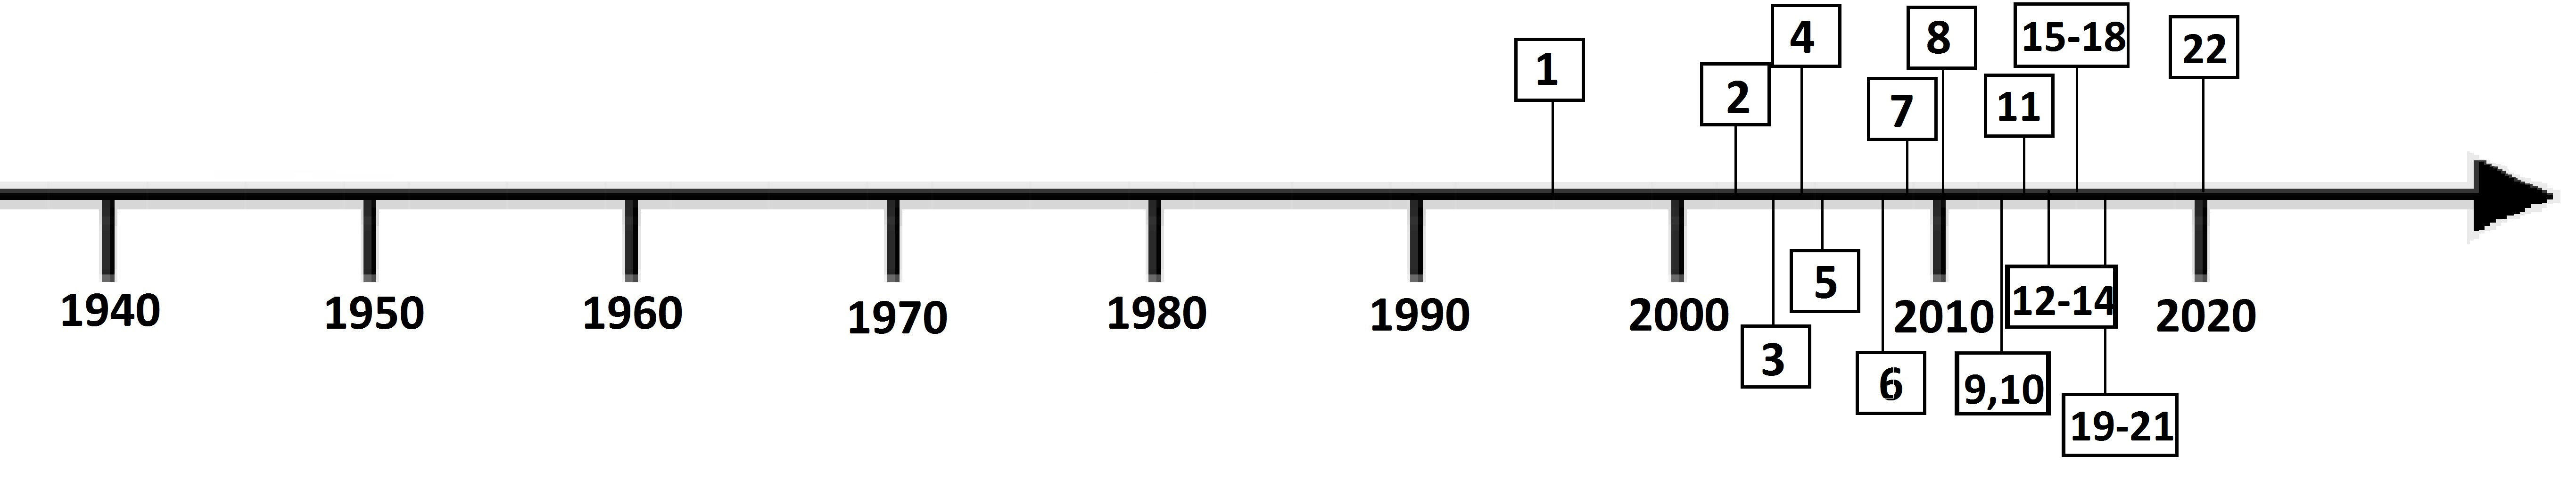
\includegraphics[width=\textwidth]{Kapitel/5G/Grafiken/Zeitstrahl}
\par
\noindent
\begin{tabular}{|p{1 cm}|p{3 cm}|p{13.55 cm}|}
	\hline
	Nummer & Datum & Entwicklungsschritte~\cite{5g.1}\\
	\hline
	1 & 1996 & 2G GSM \\
	\hline
	2 & 2002 & Bekanntgabe der strategischen Vision für 4G\cite{5g.5} \\
	\hline
	3 & 2004 & 3G UMTS\\
	\hline 
	4 & Anfang 2005 & Beginn der Standardisierung von 4G\cite{5g.5} \\
	\hline
	5 & 2006 & 3G HSPA\\
	\hline
	6 & 2008 & Die ersten Entwicklungsgruppen für 5G Mobilkommunikationssysteme werden gebildet.\\
	\hline
	7 & 2009 & Das erste kommerzielle 4G-Netz wird von Ericsson und TeliaSonera in Betrieb genommen. \\
	\hline
	8 & 2010 & 4G LTE großflächig verbreitet \\
	\hline
	9 & 8. Oktober 2012 & Es erfolgt die Gründung eines 5G-Forschungszentrum an der Universität in Surrey, Großbritannien. \\
	\hline
	10 & November 2012 & Das \textit{iJOIN}-EU-Projektes zur Erforschung der besseren Ausnutzung des Spektrums wird gestartet. \\
	\hline
	11 & 12. Mai 2013 & Samsung verkündet, das erste 5G-System entwickelt zu haben, welches Geschwindigkeiten bis zu 10Gbit/s erreichen können soll. Im Test wurde bei einer Reichweite von 2km eine Geschwindigkeit von 1.056Gbits erreicht. \\
	\hline
	12 & 8. Mai 2014 & NTT DoCoMo beginnt 5G-Tests in Kooperation mit Alcatel, Ericsson, Fujistu, NEC, Nokia und Samsung. \\
	\hline
	13 & Oktober 2014 & Das Projekt TIGRE5-CM wird gestartet, um die Architektur von künftigen Mobilfunknetzen auf Basis von SDN-Paradigmen (Software-defining networking) zu entwerfen. \\
	\hline
	14 & November 2014 & Huawei und Megafon beginnen in Russland mit der Entwicklung eines 5G-Netzwerkes. Ein Testnetz soll bis Ende 2017 entstehen. \\
	\hline
	15 & März 2015 & Vorstellung erster Ergebnisse des iJOIN-Projektes auf dem Mobile World Congress 2015 \\
	\hline
	16 & September 2015 & Das 3rd Generation Partnership Project, kurz 3GPP, hält eine Konferenz zur Diskussion über die Entwicklung eines 5G-Standards ab. \\
	\hline
	17 & 8. September 2015 & Verizon gibt bekannt, dass 2016 erste Tests von 5G in den USA beginnen sollen. \\
	\hline
	18 & 28. September 2015 & Telekom gibt bekannt, dass ein erster Test mit SIC erfolgreich war, sodass zum ersten Mal IBFD erreicht wurde. \cite{5g.2} \\
	\hline
	19 & 22. Januar 2016 & Ericsson und TeliaSonera geben erneut eine Zusammenarbeit bekannt. Sie wollen 2018 in Stockholm, Schweden, und in Tallinn, Estland, die ersten 5G-Services anbieten. \\
	\hline
	20 & 22. Februar 2016 & Samsung und Verizon geben ihre Zusammenarbeit bei 5G-Tests bekannt. \\
	\hline
	21 & 23. Februar 2016 & Telekom führt auf dem Mobile World Congress 2016 einen 5G-Prototypen mit einer Geschwindigkeit von 1,5Gbits und weniger als 1ms Latenzzeit vor. \cite{5g.4}\\
	\hline
	22 & 2020 & geplantes großflächiges Einführungsjahr der Technik \\
	\hline
\end{tabular}
\par
\begin{multicols}{3}
\begin{Figure}
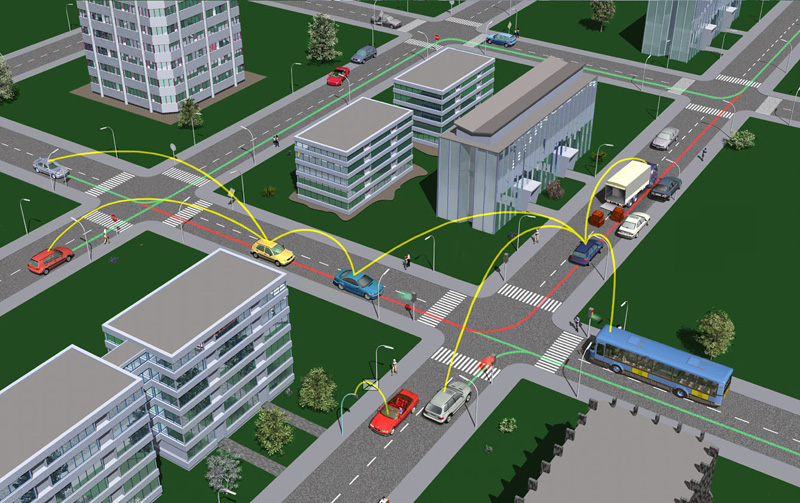
\includegraphics[width=\linewidth]{Kapitel/5G/Grafiken/c2c}
\captionof{figure}{3D Car-2-Car-Scenario von BMW ~\cite{5g.11}}
\label{fig:5g.c2c}
\end{Figure}

In der Medizin könnten diese Latenzzeiten in Kombination mit extrem präziser VR ermöglichen, dass spezialisierte Ärzte Operationen ausführen, obwohl sie sich an einem vollkommen anderen Ort in der Welt befinden. Dies kann zum Beispiel bei besonders schweren und komplizierten Operationen genutzt werden, die nur von wenigen Chirurgen präzise beherrscht werden.\cite{5g.10}
\subsection*{Ausblick}
Wenn wir den Ankündigungen der führenden Firmen glauben, so soll 5G ab 2020 im Einsatz sein. Ab dem Gründung der ersten Forschungszentren für die Technik wären zu diesem Zeitpunkt also 8 Jahre vergangen.
Dies entspricht auch der Zeit, die es bei 4G von der strategischen Version 2002 bis zum Praxisbetrieb 2010 benötigt hat, weshalb es durchaus realistisch ist, dass 5G tatsächlich 2020 einsatzbereit ist. 
Mit dem Aufkommen von 5G stehen dann sowohl der Wirtschaft, in Bereichen wie Smart Logistics, als auch dem Endverbraucher, durch Dinge wie selbstfahrende Autos und Health Monitoring, ganz neue Möglichkeiten zur Verfügung, die das Leben verbessern können.

\printbibliography[segment=10,heading=subbibliography]
\end{multicols}

\newpage
